% questions.tex —— 1977 年·安徽卷（文科） · 题目内容片段（无答案）
% 由 tools/generate_projects.py 依来源总账自 1977/1977_数学真题_安徽文_试题.md 生成，勿手改（改源 MD 后重跑）


\gkpart{数学试卷（安徽卷·文科）}

\begin{gktip}
\textbf{来源说明}：本题面依据固定源 PDF《1977安徽文.pdf》第 1—3 页逐题转录，正式题共 10 道，无附加题、参考题；第 4—10 页为同一 PDF 所附《解答和评分标准》（题面页带书籍页码 55—56，解答页带书籍页码 29—35「题解」），不是无答案试卷。原卷大题以汉数字「一、」至「十、」编号，第 1、2 题的小项印作「1．」至「5．」「1．」「2．」，本库按规范将大题重排为阿拉伯数字 1—10、小项重排为（1）（2）……，未增删题干；第 1 题引语「计算」在原卷与首个小项排印同行，现独立成行。原卷正切记作「tg」、余弦有一处排作首字母大写的「Cos」，均按原样保留（数学式中排作反斜杠 operatorname 形式）；小写「sin」按标准函数记号排印。
\end{gktip}

\par\medskip

\begin{question}
\gkti{1}\textbf{（本题25分，每小题5分）} 

计算

（1） $5\frac{1}{2}\times\left(-\dfrac{6}{11}\right)+0.25-(-2)^3\div\left(-2\frac{2}{3}\right)^2$；

（2） $\sqrt{14\times24\times39\times91}+4\sqrt{27}\times(-\sqrt3)$；

（3） $\left(-2\frac{3}{5}\right)^0+4^{-2}\times\left(2\frac{1}{4}\right)^{-\frac{1}{2}}-(0.01)^{0.5}$；

（4） $\dfrac{2\lg2+\lg3}{2+\lg0.36+\dfrac{2}{3}\lg8}$；

（5） $\dfrac{\operatorname{tg}(-120^\circ)\cdot\operatorname{Cos}(-240^\circ)\cdot\operatorname{Cos}480^\circ}{\operatorname{tg}(-60^\circ)\cdot\sin(-1050^\circ)}$。

\end{question}
\begin{question}
\gkti{2}\textbf{（本题满分10分，每小题5分）} 

化简；

（1） $\left(3\sqrt[3]{a^2}\cdot\sqrt{b}\right)\cdot\left(-6\sqrt{a}\cdot\sqrt[3]{b}\right)\div\left(-2\sqrt[6]{a}\cdot\sqrt[6]{b^5}\right)$；

（2） $\sqrt{(\lg x)^2-2\lg x+1}$。

\end{question}
\begin{question}
\gkti{3}\textbf{（满分5分）} 分解因式

\nopagebreak[4]
\[
a^2-2ab+b^2-6a+6b+5.
\]

\end{question}
\begin{question}
\gkti{4}\textbf{（满分10分，每小题5分）} 

求下列函数的定义域，并在数轴上把它们表示出来：

（1） $y=\dfrac{\sqrt{3+2x}}{3x-1}$；

（2） $y=\arcsin\dfrac{x}{3}$。

\end{question}
\begin{question}
\gkti{5}\textbf{（本题8分）} 

\Needspace{5\baselineskip}
求证

\nopagebreak[4]
\[
\frac{\sin\alpha+\sin\beta}{\sin(\alpha+\beta)}
=\frac{\operatorname{Cos}\dfrac{\alpha-\beta}{2}}{\operatorname{Cos}\dfrac{\alpha+\beta}{2}}.
\]

\end{question}
\begin{question}
\gkti{6}\textbf{（本题8分）} 

\Needspace{5\baselineskip}
解方程

\nopagebreak[4]
\[
\sin x+\operatorname{Cos}x-1=0.
\]

\end{question}
\begin{question}
\gkti{7}\textbf{（本题8分）} 

\Needspace{5\baselineskip}
求下列等式里的实数 $x$ 和 $y$ 的值：

\nopagebreak[4]
\[
(3xi+2x)+(yi-4)=(2y+5i)-(3+xi).
\]

\Needspace{0.4\textheight}
\end{question}
\begin{question}
\gkti{8}\textbf{（本题8分）} 

从山顶 $D$ 测得地面上同一方向的两点 $A$ 和 $B$ 的俯角分别是 $30^\circ$ 和 $45^\circ$，已知 $AB=40$ 米，求山高（精确到 $0.1$）。

\begin{gktip}
原源 PDF 第 2 页附有山顶俯角测高示意图；LaTeX 版按源图重绘。
\end{gktip}
\nopagebreak[4]
\begin{center}% 1977 年安徽卷（文科）第 8 题：山顶 D 测山高示意图（按源卷布局）
% DC 垂直于基线 AC（直角在 C，原图未画直角标记），过 D 水平虚线；
% 俯角 30° 弧（水平线到 DA）与 45° 弧（水平线到 DB）标在 D 处，
% 45° 标签按原图写在视线 DA 与 DB 之间。
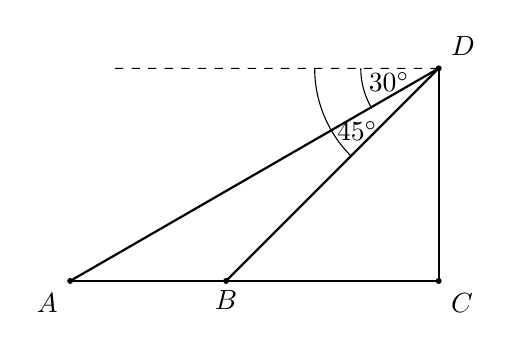
\begin{tikzpicture}[scale=0.9, line join=round]
  \coordinate (A) at (-5.2,0);
  \coordinate (B) at (-3,0);
  \coordinate (C) at (0,0);
  \coordinate (D) at (0,3);
  \draw[thick] (A) -- (C);
  \draw[thick] (C) -- (D);
  \draw[thick] (D) -- (A);
  \draw[thick] (D) -- (B);
  \draw[dashed] (D) -- (-4.6,3);
  \fill (A) circle (1.2pt) node[below left=1pt] {$A$};
  \fill (B) circle (1.2pt) node[below] {$B$};
  \fill (C) circle (1.2pt) node[below right=1pt] {$C$};
  \fill (D) circle (1.2pt) node[above right=1pt] {$D$};
  \draw (-1.1,3) arc[start angle=180, end angle=210, radius=1.1];
  \draw (-1.75,3) arc[start angle=180, end angle=225, radius=1.75];
  \node at (-0.70,2.81) {$30^\circ$};
  \node at (-1.15,2.12) {$45^\circ$};
\end{tikzpicture}
\end{center}
\nopagebreak[4]
\end{question}
\begin{question}
\gkti{9}\textbf{（本题8分）} 

红旗大队粮食产量逐年增加，1973年产量为90万斤，连续三年平均每年比前一年增产10\%，这个大队从1973年到1976年总共生产粮食多少万斤？（精确到0.1）

\end{question}
\begin{question}
\gkti{10}\textbf{（本题10分）} 

求椭圆 $25x^2+9y^2=100$ 的长轴和短轴的长、焦点坐标，并且画出它的图象。

\end{question}